\documentclass[11pt]{article}
\title{Technical Report\\ COMP1100 Assignment 2}
\author{Jacob Bos\\ ANU u7469354}

\usepackage{graphicx}
\usepackage{amsmath}
\usepackage{amssymb}
\usepackage{array}
	\newcolumntype{L}{>{\centering\arraybackslash}m{15cm}}
\usepackage{float}
\usepackage{multicol}
\setlength{\columnsep}{1cm}
\usepackage{setspace}
\usepackage{xcolor}

\newenvironment{smallpmatrix}
  {\left(\begin{smallmatrix}}
  {\end{smallmatrix}\right)}
 \newenvironment{smol}
  {\left(\begin{smallmatrix}}
  {\end{smallmatrix}\right)}


\usepackage[margin=2cm]{geometry}
\addtolength{\textheight}{-0.5cm}
%~~~~~~~~~~~~~~~~~~~~~~~~~~~~~~~~~~~~~~~~~~~~~~~~~~~~~~~~~~~~~~~~~~~~~~~~~~~~~~~~~~~~~~~~~~~~~~~~~~~~
%~~~~~~~~~~~~~~~~~~~~~~~~~~~~~~~~~~~~~~~~~~~~~~~~~~~~~~~~~~~~~~~~~~~~~~~~~~~~~~~~~~~~~~~~~~~~~~~~~~~~
\begin{document}
\maketitle
\pagenumbering{roman}
\setstretch{1.5}
\begin{center}
  Lab: Tuesday 11am\\
  Tutor: Abhaas Goyal\\
  Word-count beyond cover page at $\leq 1250$ words
\end{center}
\tableofcontents
\newpage
\pagenumbering{arabic}
%~~~~~~~~~~~~~~~~~~~~~~~~~~~~~~~~~~~~~~~~~~~~~~~~~~~~~~~~~~~~~~~~~~~~~~~~~~~~~~~~~~~~~~~~~~~~~~~~~~~~
\section{Introduction} 
The program detailed in this report is an implementation of Erik Fransson's \textit{QR World} cellular automata with a graphical representation in Haskell. The automata is contained within a module called \verb|Automata| with user input handling in module \verb|App| and graphical output handled in \verb|GridRenderer|. Testing is handled by three modules with unit tests within \verb|AutomataTest|.


%~~~~~~~~~~~~~~~~~~~~~~~~~~~~~~~~~~~~~~~~~~~~~~~~~~~~~~~~~~~~~~~~~~~~~~~~~~~~~~~~~~~~~~~~~~~~~~~~~~~~
\section{Documentation}%Explanation of code workings, functions and structure.
\subsection{Design Documentation and Technical Decisions}
% Describe what each relevant function does conceptually. (i.e. how does it get you closer to solving the problems outlined in this assignment spec?)
% How do these functions piece together to make the finished program? Why did you design and implement it this way?
% What major design choices did you make regarding the functions that you’ve written and the overall structure of your program?
\paragraph{Task 1} consists of 5 functions. The type of \verb|QRCell| is defined as either \verb|Dead| or \verb|Alive|. An if then else (ITE) statement was used for \verb|toQR| to convert values in the textual representation to useful values with \verb|'A'| to \verb| Alive::QRCell| and any other characters as \verb|Dead|.  \verb|cycleQR| swaps the value of a cell upon cursor clicks using a case statement.  If \verb|type QRCell = Bool| then the function could just be \verb|not|. \verb|renderQR| renders each cell as the specified codeWorld picture.  \verb|get| retrieves the value of the model at a given \verb|GridCoord|, returning \verb|Nothing| for nonsensical arguments. \verb|allCoords| generates a row-major list of all grid coordinates in an $a\times b$ for $a,b>0$ grid.  It returns an error for nonsensical arguments of $a,b\not>0$ as par specifications. Otherwise it calls 3 helper functions. \verb|nList| generates an ascending list from 0 to (a-1). \verb|nPair| then pairs each value in the \verb|nList| with some integer. \verb|allPairs| then does this to create one list from (0,0) to (a-1,b-1). 

\paragraph{Task 2} consists of two primary functions, \verb|nextGenQR| which parses the automata through one iteration, and \verb|evolveQR| which iterates the automata $n$ times. \verb|nextGenQR| calls the helper functions \verb|allCoords| and \verb|nextGenQrGrid| which is the main function handling the evolution of the grid. \verb|nextGenQrGrid| recurses through the \verb|allCoords| list using \verb|get| to retrieve the state at each position and the helper \verb|findHood| to retrieve a list of the states of the four neighbors. The helper \verb|decideEvolve| then chooses updates the state of the cell according to the QRWorld rules. This new state is then prepended to the recursive call on the rest of the list.  \verb|allCoords| is guarded to return an error for nonsensical grid dimensions to avoid irrational program operation. A guarded case recursion was chosen for \verb|countAlive| to only count specific elements. \verb|decideEvolve| was chosen to use a case to direct the function to guards based on the number of alive neighbours determined by \verb|countAlive| to then decide how to change  the state. \verb|findHood| uses \verb|get| to retrieve a four element list of \verb|[Maybe QRCell]| to give the states of the neighbouring cells. \verb|decideEvolve| then calls \verb|countAlive| to then make a decision about what each cell state should evolve to depending on how many alive neighbours it has. To do this it cases on the state of the cell and is then guarded by the number of alives to evolve the state properly. \verb|countAlive| just uses a case and nested guard recursion to sort through the list of neighboring states and returns the number that are alive. \verb|evolveQR| recurses down to a base of 1 from a natural $n$ applying \verb|nextGenQR| to itself $n$ times.


 \subsection{Assumptions}%Describe assumptions you have made about how a user might use the program and how this has influenced your design decisions.
Whilst writing \verb|get| it was assumed that attempts to retrieve a point outside the grid should return \verb|Nothing :: Maybe QRCell| as doing so eased implementation of \verb|findHood| and \verb|countAlive| far more than returning an error would. It was initially assumed that nonsensical inputs to \verb|allCoords| should return an empty list but this was revised to return an error as specified.

%~~~~~~~~~~~~~~~~~~~~~~~~~~~~~~~~~~~~~~~~~~~~~~~~~~~~~~~~~~~~~~~~~~~~~~~~~~~~~~~~~~~~~~~~~~~~~~~~~~~~

\section{Testing}%How did I test the program focus on methodology and testing groups
%How did you test individual functions?
%Be specific about this - the tutors know that you have tested your program, but they want to know how.
%Describe the tests that prove individual functions on their own behave as expected (i.e. testing a function with different inputs and doing a calculation by hand to check that the outputs are correct).
%How did you test the entire program? What tests did you perform to show that the program behaves as expected in all (even unusual) cases?
\paragraph{Unit tests} were divided into 6 groups: cycleQRTests, getTests, allCoordsTest, toQRTests, evolveQRTests and countAliveTests. Each test group tests a particular function or group of functions. \verb|cycleQRTests| is a fully comprehensive test group for \verb|cycleQR| indicating its correctness. \verb|toQR| is tested against tests two typical cases and an edge case. The tests for \verb|get| cover most possible edge cases and also some typical cases as documented in the \verb|AutomataTest| file. The tests for \verb|allCoords| covers some expected inputs to both the main function and helpers. There were no edge case tests written as such cases are written to return an error and there was no provision to test if an error is returned.\\

 \verb|evolveQR| was tested with three unit tests which in turn test \verb|nextGenQR| due to their dependencies. The first two tests tested if the 1100 pattern would get to an alternating steady state after 12 evolutions and the third if the 1130 pattern reached steady state eventually as specified. All tests passed indicating program correctness. All these tests are documented with comments in \verb|AutomataTest.hs|
\paragraph{GUI tests} focussed on the behaviour of functions that the user directly interacts with. \verb|get| and \verb|cycleQR| were tested by clicking cells with various states and checking if the appropriate cell switched state. \verb|decideEvolve| was tested by observing the evolution of a single cell in various neighbourhoods compared against the rules of QRWorld. All tests passed indicating program correctness.
%~~~~~~~~~~~~~~~~~~~~~~~~~~~~~~~~~~~~~~~~~~~~~~~~~~~~~~~~~~~~~~~~~~~~~~~~~~~~~~~~~~~~~~~~~~~~~~~~~~
\newpage
\section{Program Design / Structure}
The program and the test program have module and function dependencies according to the following graph: 
  \begin{figure}[H]
    \centering
    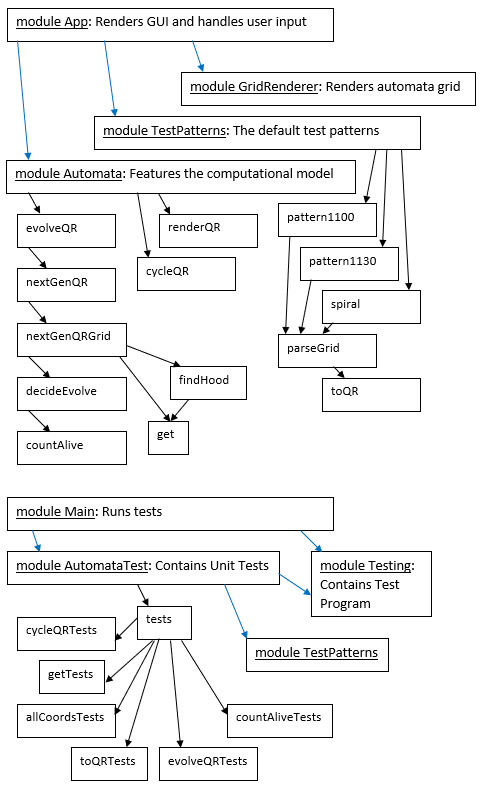
\includegraphics[width=0.65\textwidth]{funcDep.png}
  \end{figure}

  \verb|allCoords| is broken up into helper functions for ease of understanding.



\section{Reflection}
%Discuss the reasoning behind your decisions, rather than what the decisions were. You can reflect on not only the decisions you made, but the process through which you developed the final program:
   %What would you have done differently if you were to do it again
    %What changes to the design and structure you would make if you wrote the program again from scratch?
    \subsection{Design Choices}
   Development of the program followed a linear process parallel to order of assignment specifications.  Design decisions were made with both functionality and style in focus to make proper use of Haskell's recursive propensity. Consequently, program is quite readable especially due to its effective documentation comments. Many of the design decisions are detailed in Section 1.1.\\
   
   Generally ITE statements were used whenever it was necessary to only check for one case and anything else returning the same answer. As detailed, guard and case recursion was selected based on whether the function needed to iterate n times or traverse a list. When iterating n times (++) was used to order the list properly as n counts down but the list counts up. When traversing a list (:) was used to maintain the input ordering. Guard based recursion with the (++) operation was chosen for \verb|allPairs| and \verb|nList| getting the lists in ascending order. Case based (:) recursion was used for \verb|nPair| to maintain the list. \\
   
   An algebraic datatype was chosen for \verb|QRCell| as it was more descriptive of the program's meaning than boolean values. \verb|renderQR| uses a piecewise definition to improve style. Guards were chosen for \verb|get| to protect against retrieving elements outside the automata grid.  It was chosen for \verb|nextGenQR| to call \verb|nextGenQrGrid| so that the helper functions could be called appropriately and allow for a recursion through the list of \verb|allCoords|.

   \subsection{Reflection}
   If they were to re-develop the program the author believes they could rewrite or remove the helper  \verb|nPair| by using \verb|map| and the anonymous function \verb|(\y x -> (x,y))|. However, they would make no changes to the structure which was dictated largely by the specifications.\\
   
   The program was within the authors technical abilities and so there were no significant problems encountered however, the author suspects that there is a better way to write \verb|allCoords| as it is rather convoluted but other than the above mentioned, inspiration escapes them. The author had some trouble defining the type \verb|QRCell| but came to a good solution under closer reading if the specifications which allowed the rest of the program to develop smoothly. Consequently, they did not need to collaborate with others in any significant way.




%~~~~~~~~~~~~~~~~~~~~~~~~~~~~~~~~~~~~~~~~~~~~~~~~~~~~~~~~~~~~~~~~~~~~~ ~~~~~~~~~~~~~~~~~~~~~~~~~~~~~~~


%~~~~~~~~~~~~~~~~~~~~~~~~~~~~~~~~~~~~~~~~~~~~~~~~~~~~~~~~~~~~~~~~~~~~~~~~~~~~~~~~~~~~~~~~~~~~~~~~~~~~
\end{document}